
% Default to the notebook output style

    


% Inherit from the specified cell style.




    
\documentclass[11pt]{article}

    
    
    \usepackage[T1]{fontenc}
    % Nicer default font (+ math font) than Computer Modern for most use cases
    \usepackage{mathpazo}

    % Basic figure setup, for now with no caption control since it's done
    % automatically by Pandoc (which extracts ![](path) syntax from Markdown).
    \usepackage{graphicx}
    % We will generate all images so they have a width \maxwidth. This means
    % that they will get their normal width if they fit onto the page, but
    % are scaled down if they would overflow the margins.
    \makeatletter
    \def\maxwidth{\ifdim\Gin@nat@width>\linewidth\linewidth
    \else\Gin@nat@width\fi}
    \makeatother
    \let\Oldincludegraphics\includegraphics
    % Set max figure width to be 80% of text width, for now hardcoded.
    \renewcommand{\includegraphics}[1]{\Oldincludegraphics[width=.8\maxwidth]{#1}}
    % Ensure that by default, figures have no caption (until we provide a
    % proper Figure object with a Caption API and a way to capture that
    % in the conversion process - todo).
    \usepackage{caption}
    \DeclareCaptionLabelFormat{nolabel}{}
    \captionsetup{labelformat=nolabel}

    \usepackage{adjustbox} % Used to constrain images to a maximum size 
    \usepackage{xcolor} % Allow colors to be defined
    \usepackage{enumerate} % Needed for markdown enumerations to work
    \usepackage{geometry} % Used to adjust the document margins
    \usepackage{amsmath} % Equations
    \usepackage{amssymb} % Equations
    \usepackage{textcomp} % defines textquotesingle
    % Hack from http://tex.stackexchange.com/a/47451/13684:
    \AtBeginDocument{%
        \def\PYZsq{\textquotesingle}% Upright quotes in Pygmentized code
    }
    \usepackage{upquote} % Upright quotes for verbatim code
    \usepackage{eurosym} % defines \euro
    \usepackage[mathletters]{ucs} % Extended unicode (utf-8) support
    \usepackage[utf8x]{inputenc} % Allow utf-8 characters in the tex document
    \usepackage{fancyvrb} % verbatim replacement that allows latex
    \usepackage{grffile} % extends the file name processing of package graphics 
                         % to support a larger range 
    % The hyperref package gives us a pdf with properly built
    % internal navigation ('pdf bookmarks' for the table of contents,
    % internal cross-reference links, web links for URLs, etc.)
    \usepackage{hyperref}
    \usepackage{longtable} % longtable support required by pandoc >1.10
    \usepackage{booktabs}  % table support for pandoc > 1.12.2
    \usepackage[inline]{enumitem} % IRkernel/repr support (it uses the enumerate* environment)
    \usepackage[normalem]{ulem} % ulem is needed to support strikethroughs (\sout)
                                % normalem makes italics be italics, not underlines
    

    
    
    % Colors for the hyperref package
    \definecolor{urlcolor}{rgb}{0,.145,.698}
    \definecolor{linkcolor}{rgb}{.71,0.21,0.01}
    \definecolor{citecolor}{rgb}{.12,.54,.11}

    % ANSI colors
    \definecolor{ansi-black}{HTML}{3E424D}
    \definecolor{ansi-black-intense}{HTML}{282C36}
    \definecolor{ansi-red}{HTML}{E75C58}
    \definecolor{ansi-red-intense}{HTML}{B22B31}
    \definecolor{ansi-green}{HTML}{00A250}
    \definecolor{ansi-green-intense}{HTML}{007427}
    \definecolor{ansi-yellow}{HTML}{DDB62B}
    \definecolor{ansi-yellow-intense}{HTML}{B27D12}
    \definecolor{ansi-blue}{HTML}{208FFB}
    \definecolor{ansi-blue-intense}{HTML}{0065CA}
    \definecolor{ansi-magenta}{HTML}{D160C4}
    \definecolor{ansi-magenta-intense}{HTML}{A03196}
    \definecolor{ansi-cyan}{HTML}{60C6C8}
    \definecolor{ansi-cyan-intense}{HTML}{258F8F}
    \definecolor{ansi-white}{HTML}{C5C1B4}
    \definecolor{ansi-white-intense}{HTML}{A1A6B2}

    % commands and environments needed by pandoc snippets
    % extracted from the output of `pandoc -s`
    \providecommand{\tightlist}{%
      \setlength{\itemsep}{0pt}\setlength{\parskip}{0pt}}
    \DefineVerbatimEnvironment{Highlighting}{Verbatim}{commandchars=\\\{\}}
    % Add ',fontsize=\small' for more characters per line
    \newenvironment{Shaded}{}{}
    \newcommand{\KeywordTok}[1]{\textcolor[rgb]{0.00,0.44,0.13}{\textbf{{#1}}}}
    \newcommand{\DataTypeTok}[1]{\textcolor[rgb]{0.56,0.13,0.00}{{#1}}}
    \newcommand{\DecValTok}[1]{\textcolor[rgb]{0.25,0.63,0.44}{{#1}}}
    \newcommand{\BaseNTok}[1]{\textcolor[rgb]{0.25,0.63,0.44}{{#1}}}
    \newcommand{\FloatTok}[1]{\textcolor[rgb]{0.25,0.63,0.44}{{#1}}}
    \newcommand{\CharTok}[1]{\textcolor[rgb]{0.25,0.44,0.63}{{#1}}}
    \newcommand{\StringTok}[1]{\textcolor[rgb]{0.25,0.44,0.63}{{#1}}}
    \newcommand{\CommentTok}[1]{\textcolor[rgb]{0.38,0.63,0.69}{\textit{{#1}}}}
    \newcommand{\OtherTok}[1]{\textcolor[rgb]{0.00,0.44,0.13}{{#1}}}
    \newcommand{\AlertTok}[1]{\textcolor[rgb]{1.00,0.00,0.00}{\textbf{{#1}}}}
    \newcommand{\FunctionTok}[1]{\textcolor[rgb]{0.02,0.16,0.49}{{#1}}}
    \newcommand{\RegionMarkerTok}[1]{{#1}}
    \newcommand{\ErrorTok}[1]{\textcolor[rgb]{1.00,0.00,0.00}{\textbf{{#1}}}}
    \newcommand{\NormalTok}[1]{{#1}}
    
    % Additional commands for more recent versions of Pandoc
    \newcommand{\ConstantTok}[1]{\textcolor[rgb]{0.53,0.00,0.00}{{#1}}}
    \newcommand{\SpecialCharTok}[1]{\textcolor[rgb]{0.25,0.44,0.63}{{#1}}}
    \newcommand{\VerbatimStringTok}[1]{\textcolor[rgb]{0.25,0.44,0.63}{{#1}}}
    \newcommand{\SpecialStringTok}[1]{\textcolor[rgb]{0.73,0.40,0.53}{{#1}}}
    \newcommand{\ImportTok}[1]{{#1}}
    \newcommand{\DocumentationTok}[1]{\textcolor[rgb]{0.73,0.13,0.13}{\textit{{#1}}}}
    \newcommand{\AnnotationTok}[1]{\textcolor[rgb]{0.38,0.63,0.69}{\textbf{\textit{{#1}}}}}
    \newcommand{\CommentVarTok}[1]{\textcolor[rgb]{0.38,0.63,0.69}{\textbf{\textit{{#1}}}}}
    \newcommand{\VariableTok}[1]{\textcolor[rgb]{0.10,0.09,0.49}{{#1}}}
    \newcommand{\ControlFlowTok}[1]{\textcolor[rgb]{0.00,0.44,0.13}{\textbf{{#1}}}}
    \newcommand{\OperatorTok}[1]{\textcolor[rgb]{0.40,0.40,0.40}{{#1}}}
    \newcommand{\BuiltInTok}[1]{{#1}}
    \newcommand{\ExtensionTok}[1]{{#1}}
    \newcommand{\PreprocessorTok}[1]{\textcolor[rgb]{0.74,0.48,0.00}{{#1}}}
    \newcommand{\AttributeTok}[1]{\textcolor[rgb]{0.49,0.56,0.16}{{#1}}}
    \newcommand{\InformationTok}[1]{\textcolor[rgb]{0.38,0.63,0.69}{\textbf{\textit{{#1}}}}}
    \newcommand{\WarningTok}[1]{\textcolor[rgb]{0.38,0.63,0.69}{\textbf{\textit{{#1}}}}}
    
    
    % Define a nice break command that doesn't care if a line doesn't already
    % exist.
    \def\br{\hspace*{\fill} \\* }
    % Math Jax compatability definitions
    \def\gt{>}
    \def\lt{<}
    % Document parameters
    \title{index}
    
    
    

    % Pygments definitions
    
\makeatletter
\def\PY@reset{\let\PY@it=\relax \let\PY@bf=\relax%
    \let\PY@ul=\relax \let\PY@tc=\relax%
    \let\PY@bc=\relax \let\PY@ff=\relax}
\def\PY@tok#1{\csname PY@tok@#1\endcsname}
\def\PY@toks#1+{\ifx\relax#1\empty\else%
    \PY@tok{#1}\expandafter\PY@toks\fi}
\def\PY@do#1{\PY@bc{\PY@tc{\PY@ul{%
    \PY@it{\PY@bf{\PY@ff{#1}}}}}}}
\def\PY#1#2{\PY@reset\PY@toks#1+\relax+\PY@do{#2}}

\expandafter\def\csname PY@tok@w\endcsname{\def\PY@tc##1{\textcolor[rgb]{0.73,0.73,0.73}{##1}}}
\expandafter\def\csname PY@tok@c\endcsname{\let\PY@it=\textit\def\PY@tc##1{\textcolor[rgb]{0.25,0.50,0.50}{##1}}}
\expandafter\def\csname PY@tok@cp\endcsname{\def\PY@tc##1{\textcolor[rgb]{0.74,0.48,0.00}{##1}}}
\expandafter\def\csname PY@tok@k\endcsname{\let\PY@bf=\textbf\def\PY@tc##1{\textcolor[rgb]{0.00,0.50,0.00}{##1}}}
\expandafter\def\csname PY@tok@kp\endcsname{\def\PY@tc##1{\textcolor[rgb]{0.00,0.50,0.00}{##1}}}
\expandafter\def\csname PY@tok@kt\endcsname{\def\PY@tc##1{\textcolor[rgb]{0.69,0.00,0.25}{##1}}}
\expandafter\def\csname PY@tok@o\endcsname{\def\PY@tc##1{\textcolor[rgb]{0.40,0.40,0.40}{##1}}}
\expandafter\def\csname PY@tok@ow\endcsname{\let\PY@bf=\textbf\def\PY@tc##1{\textcolor[rgb]{0.67,0.13,1.00}{##1}}}
\expandafter\def\csname PY@tok@nb\endcsname{\def\PY@tc##1{\textcolor[rgb]{0.00,0.50,0.00}{##1}}}
\expandafter\def\csname PY@tok@nf\endcsname{\def\PY@tc##1{\textcolor[rgb]{0.00,0.00,1.00}{##1}}}
\expandafter\def\csname PY@tok@nc\endcsname{\let\PY@bf=\textbf\def\PY@tc##1{\textcolor[rgb]{0.00,0.00,1.00}{##1}}}
\expandafter\def\csname PY@tok@nn\endcsname{\let\PY@bf=\textbf\def\PY@tc##1{\textcolor[rgb]{0.00,0.00,1.00}{##1}}}
\expandafter\def\csname PY@tok@ne\endcsname{\let\PY@bf=\textbf\def\PY@tc##1{\textcolor[rgb]{0.82,0.25,0.23}{##1}}}
\expandafter\def\csname PY@tok@nv\endcsname{\def\PY@tc##1{\textcolor[rgb]{0.10,0.09,0.49}{##1}}}
\expandafter\def\csname PY@tok@no\endcsname{\def\PY@tc##1{\textcolor[rgb]{0.53,0.00,0.00}{##1}}}
\expandafter\def\csname PY@tok@nl\endcsname{\def\PY@tc##1{\textcolor[rgb]{0.63,0.63,0.00}{##1}}}
\expandafter\def\csname PY@tok@ni\endcsname{\let\PY@bf=\textbf\def\PY@tc##1{\textcolor[rgb]{0.60,0.60,0.60}{##1}}}
\expandafter\def\csname PY@tok@na\endcsname{\def\PY@tc##1{\textcolor[rgb]{0.49,0.56,0.16}{##1}}}
\expandafter\def\csname PY@tok@nt\endcsname{\let\PY@bf=\textbf\def\PY@tc##1{\textcolor[rgb]{0.00,0.50,0.00}{##1}}}
\expandafter\def\csname PY@tok@nd\endcsname{\def\PY@tc##1{\textcolor[rgb]{0.67,0.13,1.00}{##1}}}
\expandafter\def\csname PY@tok@s\endcsname{\def\PY@tc##1{\textcolor[rgb]{0.73,0.13,0.13}{##1}}}
\expandafter\def\csname PY@tok@sd\endcsname{\let\PY@it=\textit\def\PY@tc##1{\textcolor[rgb]{0.73,0.13,0.13}{##1}}}
\expandafter\def\csname PY@tok@si\endcsname{\let\PY@bf=\textbf\def\PY@tc##1{\textcolor[rgb]{0.73,0.40,0.53}{##1}}}
\expandafter\def\csname PY@tok@se\endcsname{\let\PY@bf=\textbf\def\PY@tc##1{\textcolor[rgb]{0.73,0.40,0.13}{##1}}}
\expandafter\def\csname PY@tok@sr\endcsname{\def\PY@tc##1{\textcolor[rgb]{0.73,0.40,0.53}{##1}}}
\expandafter\def\csname PY@tok@ss\endcsname{\def\PY@tc##1{\textcolor[rgb]{0.10,0.09,0.49}{##1}}}
\expandafter\def\csname PY@tok@sx\endcsname{\def\PY@tc##1{\textcolor[rgb]{0.00,0.50,0.00}{##1}}}
\expandafter\def\csname PY@tok@m\endcsname{\def\PY@tc##1{\textcolor[rgb]{0.40,0.40,0.40}{##1}}}
\expandafter\def\csname PY@tok@gh\endcsname{\let\PY@bf=\textbf\def\PY@tc##1{\textcolor[rgb]{0.00,0.00,0.50}{##1}}}
\expandafter\def\csname PY@tok@gu\endcsname{\let\PY@bf=\textbf\def\PY@tc##1{\textcolor[rgb]{0.50,0.00,0.50}{##1}}}
\expandafter\def\csname PY@tok@gd\endcsname{\def\PY@tc##1{\textcolor[rgb]{0.63,0.00,0.00}{##1}}}
\expandafter\def\csname PY@tok@gi\endcsname{\def\PY@tc##1{\textcolor[rgb]{0.00,0.63,0.00}{##1}}}
\expandafter\def\csname PY@tok@gr\endcsname{\def\PY@tc##1{\textcolor[rgb]{1.00,0.00,0.00}{##1}}}
\expandafter\def\csname PY@tok@ge\endcsname{\let\PY@it=\textit}
\expandafter\def\csname PY@tok@gs\endcsname{\let\PY@bf=\textbf}
\expandafter\def\csname PY@tok@gp\endcsname{\let\PY@bf=\textbf\def\PY@tc##1{\textcolor[rgb]{0.00,0.00,0.50}{##1}}}
\expandafter\def\csname PY@tok@go\endcsname{\def\PY@tc##1{\textcolor[rgb]{0.53,0.53,0.53}{##1}}}
\expandafter\def\csname PY@tok@gt\endcsname{\def\PY@tc##1{\textcolor[rgb]{0.00,0.27,0.87}{##1}}}
\expandafter\def\csname PY@tok@err\endcsname{\def\PY@bc##1{\setlength{\fboxsep}{0pt}\fcolorbox[rgb]{1.00,0.00,0.00}{1,1,1}{\strut ##1}}}
\expandafter\def\csname PY@tok@kc\endcsname{\let\PY@bf=\textbf\def\PY@tc##1{\textcolor[rgb]{0.00,0.50,0.00}{##1}}}
\expandafter\def\csname PY@tok@kd\endcsname{\let\PY@bf=\textbf\def\PY@tc##1{\textcolor[rgb]{0.00,0.50,0.00}{##1}}}
\expandafter\def\csname PY@tok@kn\endcsname{\let\PY@bf=\textbf\def\PY@tc##1{\textcolor[rgb]{0.00,0.50,0.00}{##1}}}
\expandafter\def\csname PY@tok@kr\endcsname{\let\PY@bf=\textbf\def\PY@tc##1{\textcolor[rgb]{0.00,0.50,0.00}{##1}}}
\expandafter\def\csname PY@tok@bp\endcsname{\def\PY@tc##1{\textcolor[rgb]{0.00,0.50,0.00}{##1}}}
\expandafter\def\csname PY@tok@fm\endcsname{\def\PY@tc##1{\textcolor[rgb]{0.00,0.00,1.00}{##1}}}
\expandafter\def\csname PY@tok@vc\endcsname{\def\PY@tc##1{\textcolor[rgb]{0.10,0.09,0.49}{##1}}}
\expandafter\def\csname PY@tok@vg\endcsname{\def\PY@tc##1{\textcolor[rgb]{0.10,0.09,0.49}{##1}}}
\expandafter\def\csname PY@tok@vi\endcsname{\def\PY@tc##1{\textcolor[rgb]{0.10,0.09,0.49}{##1}}}
\expandafter\def\csname PY@tok@vm\endcsname{\def\PY@tc##1{\textcolor[rgb]{0.10,0.09,0.49}{##1}}}
\expandafter\def\csname PY@tok@sa\endcsname{\def\PY@tc##1{\textcolor[rgb]{0.73,0.13,0.13}{##1}}}
\expandafter\def\csname PY@tok@sb\endcsname{\def\PY@tc##1{\textcolor[rgb]{0.73,0.13,0.13}{##1}}}
\expandafter\def\csname PY@tok@sc\endcsname{\def\PY@tc##1{\textcolor[rgb]{0.73,0.13,0.13}{##1}}}
\expandafter\def\csname PY@tok@dl\endcsname{\def\PY@tc##1{\textcolor[rgb]{0.73,0.13,0.13}{##1}}}
\expandafter\def\csname PY@tok@s2\endcsname{\def\PY@tc##1{\textcolor[rgb]{0.73,0.13,0.13}{##1}}}
\expandafter\def\csname PY@tok@sh\endcsname{\def\PY@tc##1{\textcolor[rgb]{0.73,0.13,0.13}{##1}}}
\expandafter\def\csname PY@tok@s1\endcsname{\def\PY@tc##1{\textcolor[rgb]{0.73,0.13,0.13}{##1}}}
\expandafter\def\csname PY@tok@mb\endcsname{\def\PY@tc##1{\textcolor[rgb]{0.40,0.40,0.40}{##1}}}
\expandafter\def\csname PY@tok@mf\endcsname{\def\PY@tc##1{\textcolor[rgb]{0.40,0.40,0.40}{##1}}}
\expandafter\def\csname PY@tok@mh\endcsname{\def\PY@tc##1{\textcolor[rgb]{0.40,0.40,0.40}{##1}}}
\expandafter\def\csname PY@tok@mi\endcsname{\def\PY@tc##1{\textcolor[rgb]{0.40,0.40,0.40}{##1}}}
\expandafter\def\csname PY@tok@il\endcsname{\def\PY@tc##1{\textcolor[rgb]{0.40,0.40,0.40}{##1}}}
\expandafter\def\csname PY@tok@mo\endcsname{\def\PY@tc##1{\textcolor[rgb]{0.40,0.40,0.40}{##1}}}
\expandafter\def\csname PY@tok@ch\endcsname{\let\PY@it=\textit\def\PY@tc##1{\textcolor[rgb]{0.25,0.50,0.50}{##1}}}
\expandafter\def\csname PY@tok@cm\endcsname{\let\PY@it=\textit\def\PY@tc##1{\textcolor[rgb]{0.25,0.50,0.50}{##1}}}
\expandafter\def\csname PY@tok@cpf\endcsname{\let\PY@it=\textit\def\PY@tc##1{\textcolor[rgb]{0.25,0.50,0.50}{##1}}}
\expandafter\def\csname PY@tok@c1\endcsname{\let\PY@it=\textit\def\PY@tc##1{\textcolor[rgb]{0.25,0.50,0.50}{##1}}}
\expandafter\def\csname PY@tok@cs\endcsname{\let\PY@it=\textit\def\PY@tc##1{\textcolor[rgb]{0.25,0.50,0.50}{##1}}}

\def\PYZbs{\char`\\}
\def\PYZus{\char`\_}
\def\PYZob{\char`\{}
\def\PYZcb{\char`\}}
\def\PYZca{\char`\^}
\def\PYZam{\char`\&}
\def\PYZlt{\char`\<}
\def\PYZgt{\char`\>}
\def\PYZsh{\char`\#}
\def\PYZpc{\char`\%}
\def\PYZdl{\char`\$}
\def\PYZhy{\char`\-}
\def\PYZsq{\char`\'}
\def\PYZdq{\char`\"}
\def\PYZti{\char`\~}
% for compatibility with earlier versions
\def\PYZat{@}
\def\PYZlb{[}
\def\PYZrb{]}
\makeatother


    % Exact colors from NB
    \definecolor{incolor}{rgb}{0.0, 0.0, 0.5}
    \definecolor{outcolor}{rgb}{0.545, 0.0, 0.0}



    
    % Prevent overflowing lines due to hard-to-break entities
    \sloppy 
    % Setup hyperref package
    \hypersetup{
      breaklinks=true,  % so long urls are correctly broken across lines
      colorlinks=true,
      urlcolor=urlcolor,
      linkcolor=linkcolor,
      citecolor=citecolor,
      }
    % Slightly bigger margins than the latex defaults
    
    \geometry{verbose,tmargin=1in,bmargin=1in,lmargin=1in,rmargin=1in}
    
    

    \begin{document}
    
    
    \maketitle
    
    

    
    \section{Nearest Neighbors Lab}\label{nearest-neighbors-lab}

\subsection{Objectives}\label{objectives}

\begin{itemize}
\tightlist
\item
  Apply the nearest neighbors approach in a real world domain to answer
  similarity based analytical questions around data.
\item
  Use pandas and numpy for calculating distance based similarity
  measures between data objects.
\item
  Perform basic data exploration and feature selection for a given
  dataset.
\item
  Group and plot similarity between geographical data objects using
  folium.
\item
  Practice data manipulation between lists, dictionaries, numpy arrays
  and pandas dataframe.
\item
  Develop a complete system based on re-usable functions to perform unit
  tasks.
\end{itemize}

    \subsubsection{Introduction}\label{introduction}

In this lab, we shall apply nearest neighbors technique from previous
lab to help a taxi company predict the length of their rides. We shall
use a multitude of data types and inter-conversion between them.

Imagine that we are hired to consult for LiftOff, a limo and taxi
service that is just opening up in NYC. Liftoff wants it's taxi drivers
to target longer rides, as the longer the ride the more money it makes.
LiftOff has the following theory:

\begin{itemize}
\tightlist
\item
  \emph{The pickup location of a taxi ride can help predict the length
  of the ride.}
\end{itemize}

LiftOff asks us to do some analysis to write a function that will allow
it to \textbf{predict the length of a taxi ride for any given location
}.

Our technique will be the following: * \textbf{Collect} Obtain the data
containing all of the taxi information, and only select the attributes
of taxi trips that we need * \textbf{Explore} Examine the attributes of
our data, and plot some of our data on a map * \textbf{Train} Write our
nearest neighbors formula, and change the number of nearby trips to
predict the length of a new trip * \textbf{Predict} Use our function to
predict trip lengths of new locations

    \subsubsection{Collect and Explore the
data}\label{collect-and-explore-the-data}

    \paragraph{Collect the Data}\label{collect-the-data}

    Luckily for us, \href{https://opendata.cityofnewyork.us/}{NYC Open Data}
collects information about NYC taxi trips and provides this data on
\href{https://data.cityofnewyork.us/Transportation/2014-Yellow-Taxi-Trip-Data/gn7m-em8n}{its
website}.

    \begin{figure}
\centering
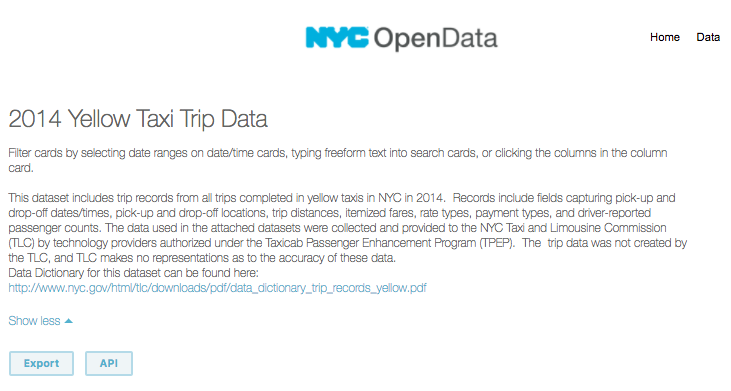
\includegraphics{./nyc-taxi.png}
\caption{}
\end{figure}

    For you're reading pleasure, the data has already been downloaded into
\texttt{trips.json} file in this lab which you can find here. We'll use
Python's \texttt{json} library to take the data from the
\texttt{trips.json} file and store it as a pandas dataframe in our
notebook. Here is the code to give you a head start.

    \begin{Verbatim}[commandchars=\\\{\}]
{\color{incolor}In [{\color{incolor}7}]:} \PY{k+kn}{import} \PY{n+nn}{pandas} \PY{k}{as} \PY{n+nn}{pd}
        \PY{k+kn}{import} \PY{n+nn}{numpy} \PY{k}{as} \PY{n+nn}{np}
        \PY{k+kn}{import} \PY{n+nn}{json}
        
        \PY{c+c1}{\PYZsh{} First, read the file}
        \PY{n}{trips\PYZus{}file} \PY{o}{=} \PY{n+nb}{open}\PY{p}{(}\PY{l+s+s1}{\PYZsq{}}\PY{l+s+s1}{trips.json}\PY{l+s+s1}{\PYZsq{}}\PY{p}{)}
        
        \PY{c+c1}{\PYZsh{} Then, convert contents to a dataframe}
        \PY{n}{trips} \PY{o}{=} \PY{n}{json}\PY{o}{.}\PY{n}{load}\PY{p}{(}\PY{n}{trips\PYZus{}file}\PY{p}{)}
        \PY{n}{trips\PYZus{}df} \PY{o}{=} \PY{n}{pd}\PY{o}{.}\PY{n}{DataFrame}\PY{p}{(}\PY{n}{trips}\PY{p}{)}
        
        \PY{n}{trips\PYZus{}df}\PY{o}{.}\PY{n}{head}\PY{p}{(}\PY{p}{)}
\end{Verbatim}


\begin{Verbatim}[commandchars=\\\{\}]
{\color{outcolor}Out[{\color{outcolor}7}]:}           dropoff\_datetime    dropoff\_latitude    dropoff\_longitude  \textbackslash{}
        0  2014-11-26T22:31:00.000  40.746769999999998  -73.997450000000001   
        1  2014-02-22T17:54:37.000  40.781844999999997           -73.979073   
        2  2014-04-06T04:07:34.000  40.726610000000001  -73.995954999999995   
        3  2014-09-08T21:15:30.000  40.773372999999999           -73.949354   
        4  2014-11-13T11:55:00.000  40.752932000000001           -73.974688   
        
          fare\_amount imp\_surcharge mta\_tax passenger\_count payment\_type  \textbackslash{}
        0          52             0     0.5               1          CSH   
        1         7.5             0     0.5               1          CSH   
        2        15.5           0.5     0.5               1          CRD   
        3        11.5           0.5     0.5               1          CSH   
        4         5.5             0     0.5               2          CRD   
        
                   pickup\_datetime     pickup\_latitude     pickup\_longitude rate\_code  \textbackslash{}
        0  2014-11-26T21:59:00.000            40.64499  -73.781149999999997         2   
        1  2014-02-22T17:47:23.000           40.766931  -73.982097999999993         1   
        2  2014-04-06T03:51:59.000  40.777729999999998  -73.951902000000004         1   
        3  2014-09-08T21:02:17.000  40.795678000000002  -73.971048999999994         1   
        4  2014-11-13T11:50:00.000           40.762912           -73.967782         1   
        
          store\_and\_fwd\_flag          tip\_amount        tolls\_amount  \textbackslash{}
        0                NaN                   0  5.3300000000000001   
        1                  N                   0                   0   
        2                  N  3.2999999999999998                   0   
        3                  N                   0                   0   
        4                NaN  1.1000000000000001                   0   
        
                 total\_amount        trip\_distance vendor\_id  
        0  57.829999999999998   18.379999999999999       VTS  
        1                   8                  1.3       CMT  
        2  19.800000000000001                  4.5       CMT  
        3                12.5   2.3999999999999999       CMT  
        4  7.0999999999999996  0.83999999999999997       VTS  
\end{Verbatim}
            
    \paragraph{Explore the data}\label{explore-the-data}

    The next step is to explore the data. First, let's see how many trips we
have.

    \begin{Verbatim}[commandchars=\\\{\}]
{\color{incolor}In [{\color{incolor}8}]:} \PY{n+nb}{len}\PY{p}{(}\PY{n}{trips\PYZus{}df}\PY{p}{)}
\end{Verbatim}


\begin{Verbatim}[commandchars=\\\{\}]
{\color{outcolor}Out[{\color{outcolor}8}]:} 1000
\end{Verbatim}
            
    1000 data elements ! , not bad at all. Now let's see what these trips
looks like. Each trip is a row in our dataframe, so we can see the
attributes of the dataframe with the \texttt{columns} function.

    \begin{Verbatim}[commandchars=\\\{\}]
{\color{incolor}In [{\color{incolor}9}]:} \PY{c+c1}{\PYZsh{} View the columns of the dataframe}
        
        \PY{n}{trips\PYZus{}df}\PY{o}{.}\PY{n}{columns}
        
        \PY{c+c1}{\PYZsh{} Index([\PYZsq{}dropoff\PYZus{}datetime\PYZsq{}, \PYZsq{}dropoff\PYZus{}latitude\PYZsq{}, \PYZsq{}dropoff\PYZus{}longitude\PYZsq{},}
        \PY{c+c1}{\PYZsh{}        \PYZsq{}fare\PYZus{}amount\PYZsq{}, \PYZsq{}imp\PYZus{}surcharge\PYZsq{}, \PYZsq{}mta\PYZus{}tax\PYZsq{}, \PYZsq{}passenger\PYZus{}count\PYZsq{},}
        \PY{c+c1}{\PYZsh{}        \PYZsq{}payment\PYZus{}type\PYZsq{}, \PYZsq{}pickup\PYZus{}datetime\PYZsq{}, \PYZsq{}pickup\PYZus{}latitude\PYZsq{},}
        \PY{c+c1}{\PYZsh{}        \PYZsq{}pickup\PYZus{}longitude\PYZsq{}, \PYZsq{}rate\PYZus{}code\PYZsq{}, \PYZsq{}store\PYZus{}and\PYZus{}fwd\PYZus{}flag\PYZsq{}, \PYZsq{}tip\PYZus{}amount\PYZsq{},}
        \PY{c+c1}{\PYZsh{}        \PYZsq{}tolls\PYZus{}amount\PYZsq{}, \PYZsq{}total\PYZus{}amount\PYZsq{}, \PYZsq{}trip\PYZus{}distance\PYZsq{}, \PYZsq{}vendor\PYZus{}id\PYZsq{}],}
        \PY{c+c1}{\PYZsh{}       dtype=\PYZsq{}object\PYZsq{})}
\end{Verbatim}


\begin{Verbatim}[commandchars=\\\{\}]
{\color{outcolor}Out[{\color{outcolor}9}]:} Index(['dropoff\_datetime', 'dropoff\_latitude', 'dropoff\_longitude',
               'fare\_amount', 'imp\_surcharge', 'mta\_tax', 'passenger\_count',
               'payment\_type', 'pickup\_datetime', 'pickup\_latitude',
               'pickup\_longitude', 'rate\_code', 'store\_and\_fwd\_flag', 'tip\_amount',
               'tolls\_amount', 'total\_amount', 'trip\_distance', 'vendor\_id'],
              dtype='object')
\end{Verbatim}
            
    \paragraph{Limit our data}\label{limit-our-data}

    We see a lot of variables in the dataset. Some of these may not be
appropriate for our analysis. Let's begin to think through what data is
relevant for our task.

    \subsubsection{Feature Selection}\label{feature-selection}

Remember that our task is to

\begin{quote}
\textbf{use the trip location to predict the length of a trip}.
\end{quote}

In order to answer above analytical question, let's select the
\texttt{pickup\_latitude}, \texttt{pickup\_longitude}, and
\texttt{trip\_distance} from each trip. That will give us the trip start
location and related \texttt{trip\_distance} for each trip. Then based
on these \textbf{actual} trip distances we can use nearest neighbors to
predict an \textbf{expected} trip distance for a new trip, provided an
\textbf{actual} location. Let's move on with this idea.

    ** Parse and Filter the dataset for required features **

    Write a function called \texttt{parse\_trips(trips)} that filters the
trips data frame and returns a new data frame containing only the
following attributes for each trip:

\begin{itemize}
\tightlist
\item
  \texttt{trip\_distance}
\item
  \texttt{pickup\_latitude}
\item
  \texttt{pickup\_longitude}
\end{itemize}

Use \texttt{dataframe.filter()} function to select above features and
create a new dataset. Make sure that all the columns in new dataset are
numeric and of type \texttt{float64}.

    \begin{Verbatim}[commandchars=\\\{\}]
{\color{incolor}In [{\color{incolor}10}]:} \PY{k}{def} \PY{n+nf}{parse\PYZus{}trips}\PY{p}{(}\PY{n}{trips}\PY{p}{)}\PY{p}{:}
             
             \PY{c+c1}{\PYZsh{} Create a new dataset containing only the required columns}
             \PY{c+c1}{\PYZsh{} Ensure the values in new dataset are numeric}
             \PY{n}{parsed} \PY{o}{=} \PY{n}{trips}\PY{o}{.}\PY{n}{filter}\PY{p}{(}\PY{p}{[}\PY{l+s+s1}{\PYZsq{}}\PY{l+s+s1}{trip\PYZus{}distance}\PY{l+s+s1}{\PYZsq{}}\PY{p}{,} \PY{l+s+s1}{\PYZsq{}}\PY{l+s+s1}{pickup\PYZus{}latitude}\PY{l+s+s1}{\PYZsq{}}\PY{p}{,} 
                                    \PY{l+s+s1}{\PYZsq{}}\PY{l+s+s1}{pickup\PYZus{}longitude}\PY{l+s+s1}{\PYZsq{}}\PY{p}{]}\PY{p}{,} \PY{n}{axis}\PY{o}{=}\PY{l+m+mi}{1}\PY{p}{)}\PY{o}{.}\PY{n}{apply}\PY{p}{(}\PY{n}{pd}\PY{o}{.}\PY{n}{to\PYZus{}numeric}\PY{p}{)}
         
             \PY{k}{return} \PY{n}{parsed}
\end{Verbatim}


    \begin{Verbatim}[commandchars=\\\{\}]
{\color{incolor}In [{\color{incolor}11}]:} \PY{n}{parsed\PYZus{}trips} \PY{o}{=} \PY{n}{parse\PYZus{}trips}\PY{p}{(}\PY{n}{trips\PYZus{}df}\PY{p}{)}
         
         \PY{n+nb}{print}\PY{p}{(}\PY{n}{parsed\PYZus{}trips}\PY{o}{.}\PY{n}{head}\PY{p}{(}\PY{p}{)}\PY{p}{,}\PY{l+s+s1}{\PYZsq{}}\PY{l+s+se}{\PYZbs{}n}\PY{l+s+s1}{\PYZsq{}}\PY{p}{,} \PY{n+nb}{type}\PY{p}{(}\PY{n}{parsed\PYZus{}trips}\PY{p}{)}\PY{p}{)}
         
         \PY{c+c1}{\PYZsh{} trip\PYZus{}distance  pickup\PYZus{}latitude  pickup\PYZus{}longitude}
         \PY{c+c1}{\PYZsh{} 0          18.38        40.644990        \PYZhy{}73.781150}
         \PY{c+c1}{\PYZsh{} 1           1.30        40.766931        \PYZhy{}73.982098}
         \PY{c+c1}{\PYZsh{} 2           4.50        40.777730        \PYZhy{}73.951902}
         \PY{c+c1}{\PYZsh{} 3           2.40        40.795678        \PYZhy{}73.971049}
         \PY{c+c1}{\PYZsh{} 4           0.84        40.762912        \PYZhy{}73.967782 }
         \PY{c+c1}{\PYZsh{} \PYZlt{}class \PYZsq{}pandas.core.frame.DataFrame\PYZsq{}\PYZgt{}}
\end{Verbatim}


    \begin{Verbatim}[commandchars=\\\{\}]
   trip\_distance  pickup\_latitude  pickup\_longitude
0          18.38        40.644990        -73.781150
1           1.30        40.766931        -73.982098
2           4.50        40.777730        -73.951902
3           2.40        40.795678        -73.971049
4           0.84        40.762912        -73.967782 
 <class 'pandas.core.frame.DataFrame'>

    \end{Verbatim}

    \subsubsection{Data Exploration and
Visualization}\label{data-exploration-and-visualization}

    Now that we have filtered our data with required columns, let's get a
sense of our trip data. We can use the \texttt{folium} Python library to
plot a map of Manhattan, and our data. First we must import
\texttt{folium}, and then use the \texttt{Map} function to pass through
a \texttt{location}, and \texttt{zoom\_start} (for current level of map
zoom - try changing it to see the effect).

\textbf{If a map isn't showing up below, copy and paste the command
\texttt{pip\ install\ folium} into your terminal to install
\texttt{folium} then try again.}

    \begin{Verbatim}[commandchars=\\\{\}]
{\color{incolor}In [{\color{incolor}34}]:} \PY{c+c1}{\PYZsh{} pip install folium}
         \PY{k+kn}{import} \PY{n+nn}{folium}
         \PY{n}{manhattan\PYZus{}map} \PY{o}{=} \PY{n}{folium}\PY{o}{.}\PY{n}{Map}\PY{p}{(}\PY{n}{location}\PY{o}{=}\PY{p}{[}\PY{l+m+mf}{40.7589}\PY{p}{,} \PY{o}{\PYZhy{}}\PY{l+m+mf}{73.9851}\PY{p}{]}\PY{p}{,} \PY{n}{zoom\PYZus{}start}\PY{o}{=}\PY{l+m+mi}{11}\PY{p}{)}
\end{Verbatim}


    \begin{Verbatim}[commandchars=\\\{\}]
{\color{incolor}In [{\color{incolor}35}]:} \PY{n}{manhattan\PYZus{}map}
\end{Verbatim}


\begin{Verbatim}[commandchars=\\\{\}]
{\color{outcolor}Out[{\color{outcolor}35}]:} <folium.folium.Map at 0x113ed0278>
\end{Verbatim}
            
    Ok, now let's see how we could add a \textbf{"marker"} to pin a specific
location using \texttt{.add\_to()} method. We'll start by getting the
map of Times Square ( {[}40.7589, -73.9851{]} ) and then putting a
marker on it.

    \begin{Verbatim}[commandchars=\\\{\}]
{\color{incolor}In [{\color{incolor}36}]:} \PY{n}{marker} \PY{o}{=} \PY{n}{folium}\PY{o}{.}\PY{n}{CircleMarker}\PY{p}{(}\PY{n}{location} \PY{o}{=} \PY{p}{[}\PY{l+m+mf}{40.7589}\PY{p}{,} \PY{o}{\PYZhy{}}\PY{l+m+mf}{73.9851}\PY{p}{]}\PY{p}{,} \PY{n}{radius}\PY{o}{=}\PY{l+m+mi}{5}\PY{p}{)}
         \PY{n}{marker}\PY{o}{.}\PY{n}{add\PYZus{}to}\PY{p}{(}\PY{n}{manhattan\PYZus{}map}\PY{p}{)}
\end{Verbatim}


\begin{Verbatim}[commandchars=\\\{\}]
{\color{outcolor}Out[{\color{outcolor}36}]:} <folium.features.CircleMarker at 0x113ed02e8>
\end{Verbatim}
            
    Above, we first create a marker. Then we add that circle marker to the
\texttt{manhattan\_map} we created earlier.

    \begin{Verbatim}[commandchars=\\\{\}]
{\color{incolor}In [{\color{incolor}37}]:} \PY{n}{manhattan\PYZus{}map}
\end{Verbatim}


\begin{Verbatim}[commandchars=\\\{\}]
{\color{outcolor}Out[{\color{outcolor}37}]:} <folium.folium.Map at 0x113ed0278>
\end{Verbatim}
            
    Do you see that blue circle near Time's Square? That is our marker.

So now that we can plot one marker on a map, we should have a sense of
how we can plot many markers on a map to display our taxi ride data. We
simply plot a map, and then we add a marker for each location of a taxi
trip.

Now let's write some functions to allow us to plot maps and add markers
a little more easily.

    \paragraph{Map plotting functions}\label{map-plotting-functions}

    As a first step towards this, note that the functions to create both a
marker and map each take in a location as two element list, representing
the latitude and longitude values. Take another look:

\begin{Shaded}
\begin{Highlighting}[]
\NormalTok{marker }\OperatorTok{=}\NormalTok{ folium.CircleMarker(location }\OperatorTok{=}\NormalTok{ [}\FloatTok{40.7589}\NormalTok{, }\OperatorTok{-}\FloatTok{73.9851}\NormalTok{])}
\NormalTok{manhattan_map }\OperatorTok{=}\NormalTok{ folium.Map(location}\OperatorTok{=}\NormalTok{[}\FloatTok{40.7589}\NormalTok{, }\OperatorTok{-}\FloatTok{73.9851}\NormalTok{])}
\end{Highlighting}
\end{Shaded}

So let's write a function called to create this two element list from a
trip. Write a function called \texttt{location} that takes in a trip as
an argument and returns a list where the first element is the latitude
and the second is the longitude. Remember that a location looks like the
following:

    \begin{Verbatim}[commandchars=\\\{\}]
{\color{incolor}In [{\color{incolor}38}]:} \PY{n}{first\PYZus{}trip} \PY{o}{=} \PY{n}{parsed\PYZus{}trips}\PY{o}{.}\PY{n}{iloc}\PY{p}{[}\PY{l+m+mi}{0}\PY{p}{]}
         \PY{n}{first\PYZus{}trip}
\end{Verbatim}


\begin{Verbatim}[commandchars=\\\{\}]
{\color{outcolor}Out[{\color{outcolor}38}]:} trip\_distance       18.38000
         pickup\_latitude     40.64499
         pickup\_longitude   -73.78115
         Name: 0, dtype: float64
\end{Verbatim}
            
    Now to writing our function.

    \begin{Verbatim}[commandchars=\\\{\}]
{\color{incolor}In [{\color{incolor}43}]:} \PY{k}{def} \PY{n+nf}{location}\PY{p}{(}\PY{n}{trip}\PY{p}{)}\PY{p}{:}
             \PY{n}{loc} \PY{o}{=} \PY{p}{[}\PY{n}{trip}\PY{p}{[}\PY{l+s+s1}{\PYZsq{}}\PY{l+s+s1}{pickup\PYZus{}latitude}\PY{l+s+s1}{\PYZsq{}}\PY{p}{]}\PY{p}{,} \PY{n}{trip}\PY{p}{[}\PY{l+s+s1}{\PYZsq{}}\PY{l+s+s1}{pickup\PYZus{}longitude}\PY{l+s+s1}{\PYZsq{}}\PY{p}{]}\PY{p}{]}
             \PY{k}{return} \PY{n}{loc}
\end{Verbatim}


    Let's pass the first trip in the dataset and see if it returns the
expected values.

    \begin{Verbatim}[commandchars=\\\{\}]
{\color{incolor}In [{\color{incolor}44}]:} \PY{n}{first\PYZus{}location} \PY{o}{=} \PY{n}{location}\PY{p}{(}\PY{n}{first\PYZus{}trip}\PY{p}{)} 
         \PY{n}{first\PYZus{}location} 
         
         \PY{c+c1}{\PYZsh{} [40.64499, \PYZhy{}73.78115]}
\end{Verbatim}


\begin{Verbatim}[commandchars=\\\{\}]
{\color{outcolor}Out[{\color{outcolor}44}]:} [40.64499, -73.78114999999998]
\end{Verbatim}
            
    Ok, now that we can turn a trip into a location, let's turn a location
into a marker. Write a function called \texttt{loc\_to\_marker} that
takes in a location (co-ordinates in the form of a list) as an argument,
and returns a folium \texttt{circleMarker} for that location. The radius
of the marker should always equal 5.

    \begin{Verbatim}[commandchars=\\\{\}]
{\color{incolor}In [{\color{incolor}49}]:} \PY{k}{def} \PY{n+nf}{loc\PYZus{}to\PYZus{}marker}\PY{p}{(}\PY{n}{location}\PY{p}{)}\PY{p}{:}
             \PY{n}{marker} \PY{o}{=} \PY{n}{folium}\PY{o}{.}\PY{n}{CircleMarker}\PY{p}{(}\PY{n}{location}\PY{p}{,} \PY{n}{radius} \PY{o}{=} \PY{l+m+mi}{5}\PY{p}{)}
             \PY{k}{return} \PY{n}{marker}
\end{Verbatim}


    Let's pass a location in the expected format and inspect the output.

    \begin{Verbatim}[commandchars=\\\{\}]
{\color{incolor}In [{\color{incolor}50}]:} \PY{n}{times\PYZus{}square\PYZus{}marker} \PY{o}{=} \PY{n}{loc\PYZus{}to\PYZus{}marker}\PY{p}{(}\PY{p}{[}\PY{l+m+mf}{40.7589}\PY{p}{,} \PY{o}{\PYZhy{}}\PY{l+m+mf}{73.9851}\PY{p}{]}\PY{p}{)}
         \PY{n}{times\PYZus{}square\PYZus{}marker}\PY{o}{.}\PY{n}{location} 
         
         \PY{c+c1}{\PYZsh{} [40.7589, \PYZhy{}73.9851]}
\end{Verbatim}


\begin{Verbatim}[commandchars=\\\{\}]
{\color{outcolor}Out[{\color{outcolor}50}]:} [40.7589, -73.9851]
\end{Verbatim}
            
    To check if our marker radius has been saved with location, we need to
use \texttt{json} library as the options for markers are stored in in
the json format. So let's look for the \texttt{radius} value in
\texttt{times\_square\_marker.options}.

    \begin{Verbatim}[commandchars=\\\{\}]
{\color{incolor}In [{\color{incolor}51}]:} \PY{n}{json}\PY{o}{.}\PY{n}{loads}\PY{p}{(}\PY{n}{times\PYZus{}square\PYZus{}marker}\PY{o}{.}\PY{n}{options}\PY{p}{)}\PY{p}{[}\PY{l+s+s1}{\PYZsq{}}\PY{l+s+s1}{radius}\PY{l+s+s1}{\PYZsq{}}\PY{p}{]} 
         
         \PY{c+c1}{\PYZsh{} 5}
\end{Verbatim}


\begin{Verbatim}[commandchars=\\\{\}]
{\color{outcolor}Out[{\color{outcolor}51}]:} 5
\end{Verbatim}
            
    That all worked well. So now that we know how to produce a single marker
for a trip, let's write a function to produce lots of markers for many
trips. We can write a function called \texttt{markers\_from\_trips} that
takes in \texttt{parsed\_trips}, and returns a list of marker objects
for each trip.

    \begin{Verbatim}[commandchars=\\\{\}]
{\color{incolor}In [{\color{incolor}52}]:} \PY{k}{def} \PY{n+nf}{markers\PYZus{}from\PYZus{}trips}\PY{p}{(}\PY{n}{trips}\PY{p}{)}\PY{p}{:}
             \PY{n}{locations} \PY{o}{=} \PY{p}{[}\PY{p}{]}
             \PY{n}{markers} \PY{o}{=} \PY{p}{[}\PY{p}{]}
             
             \PY{c+c1}{\PYZsh{} In a for loop, append latitude and logitude values from each row of \PYZsq{}trips\PYZsq{} to \PYZsq{}locations\PYZsq{}}
             \PY{k}{for} \PY{n}{index}\PY{p}{,} \PY{n}{trip} \PY{o+ow}{in} \PY{n}{trips}\PY{o}{.}\PY{n}{iterrows}\PY{p}{(}\PY{p}{)}\PY{p}{:}
                 \PY{n}{locations}\PY{o}{.}\PY{n}{append}\PY{p}{(}\PY{p}{[}\PY{n}{trip}\PY{p}{[}\PY{l+s+s1}{\PYZsq{}}\PY{l+s+s1}{pickup\PYZus{}latitude}\PY{l+s+s1}{\PYZsq{}}\PY{p}{]}\PY{p}{,} \PY{n}{trip}\PY{p}{[}\PY{l+s+s1}{\PYZsq{}}\PY{l+s+s1}{pickup\PYZus{}longitude}\PY{l+s+s1}{\PYZsq{}}\PY{p}{]}\PY{p}{]}\PY{p}{)}
            
             \PY{c+c1}{\PYZsh{} In a for loop, use values from \PYZsq{}locations\PYZsq{} and pass them to \PYZsq{}loc\PYZus{}to\PYZus{}marker\PYZsq{}. }
             \PY{c+c1}{\PYZsh{} Append the output for each iteration in }
             \PY{k}{for} \PY{n}{loc} \PY{o+ow}{in} \PY{n}{locations}\PY{p}{:}
                 \PY{n}{markers}\PY{o}{.}\PY{n}{append}\PY{p}{(}\PY{n}{loc\PYZus{}to\PYZus{}marker}\PY{p}{(}\PY{n}{loc}\PY{p}{)}\PY{p}{)}
             
             \PY{k}{return} \PY{n}{markers}
\end{Verbatim}


    \begin{Verbatim}[commandchars=\\\{\}]
{\color{incolor}In [{\color{incolor}53}]:} \PY{n}{trip\PYZus{}markers} \PY{o}{=} \PY{n}{markers\PYZus{}from\PYZus{}trips}\PY{p}{(}\PY{n}{parsed\PYZus{}trips}\PY{p}{)}
         \PY{n}{trip\PYZus{}markers}\PY{p}{[}\PY{l+m+mi}{0}\PY{p}{]}\PY{p}{,} \PY{n+nb}{len}\PY{p}{(}\PY{n}{trip\PYZus{}markers}\PY{p}{)}
         
         \PY{c+c1}{\PYZsh{} (\PYZlt{}folium.features.CircleMarker at 0x10edc9cf8\PYZgt{}, 1000)}
\end{Verbatim}


\begin{Verbatim}[commandchars=\\\{\}]
{\color{outcolor}Out[{\color{outcolor}53}]:} (<folium.features.CircleMarker at 0x113ed0588>, 1000)
\end{Verbatim}
            
    Great, so now we have a 1000 markers, one for each trip.

    \paragraph{A quick re-cap}\label{a-quick-re-cap}

Looking back at what we have achieved so far. We have a function that
creates locations, and a function that creates markers, it is time to
write a function to plot a map.

Write a function called \texttt{map\_from\_location} that, provided the
first argument of a list location and second argument an integer
representing the \texttt{zoom\_start}, returns a \texttt{folium} map the
corresponding location and \texttt{zoom\_start} attributes.

\begin{quote}
Hint: The following is how to write a map with folium:

\begin{Shaded}
\begin{Highlighting}[]
\NormalTok{folium.Map(location}\OperatorTok{=}\NormalTok{location, zoom_start}\OperatorTok{=}\NormalTok{zoom_amount)}
\end{Highlighting}
\end{Shaded}
\end{quote}

    \begin{Verbatim}[commandchars=\\\{\}]
{\color{incolor}In [{\color{incolor}57}]:} \PY{k}{def} \PY{n+nf}{map\PYZus{}from\PYZus{}location}\PY{p}{(}\PY{n}{location}\PY{p}{,} \PY{n}{zoom\PYZus{}amount}\PY{p}{)}\PY{p}{:}
             \PY{n}{loc\PYZus{}map} \PY{o}{=} \PY{n}{folium}\PY{o}{.}\PY{n}{Map}\PY{p}{(}\PY{n}{location}\PY{o}{=}\PY{n}{location}\PY{p}{,} \PY{n}{zoom\PYZus{}start}\PY{o}{=}\PY{n}{zoom\PYZus{}amount}\PY{p}{)}
             \PY{k}{return} \PY{n}{loc\PYZus{}map}
\end{Verbatim}


    \begin{Verbatim}[commandchars=\\\{\}]
{\color{incolor}In [{\color{incolor}58}]:} \PY{n}{times\PYZus{}square\PYZus{}map} \PY{o}{=} \PY{n}{map\PYZus{}from\PYZus{}location}\PY{p}{(}\PY{p}{[}\PY{l+m+mf}{40.7589}\PY{p}{,} \PY{o}{\PYZhy{}}\PY{l+m+mf}{73.9851}\PY{p}{]}\PY{p}{,} \PY{l+m+mi}{15}\PY{p}{)}
\end{Verbatim}


    Now we shall add the \texttt{time\_square\_marker}, calculated above to
this map using the format:

\begin{verbatim}
     <marker>.add_to(map)
\end{verbatim}

    \begin{Verbatim}[commandchars=\\\{\}]
{\color{incolor}In [{\color{incolor}59}]:} \PY{n}{times\PYZus{}square\PYZus{}marker}\PY{o}{.}\PY{n}{add\PYZus{}to}\PY{p}{(}\PY{n}{times\PYZus{}square\PYZus{}map}\PY{p}{)}
         \PY{n}{times\PYZus{}square\PYZus{}map}
\end{Verbatim}


\begin{Verbatim}[commandchars=\\\{\}]
{\color{outcolor}Out[{\color{outcolor}59}]:} <folium.folium.Map at 0x1143a1d30>
\end{Verbatim}
            
    Now that we have a marker and a map, now let's write a function that
adds a lot of markers to a map. Let's first create a Manhattan map with
zoom level = 13 as our base map to work on.

    \begin{Verbatim}[commandchars=\\\{\}]
{\color{incolor}In [{\color{incolor}60}]:} \PY{n}{manhattan\PYZus{}map} \PY{o}{=} \PY{n}{map\PYZus{}from\PYZus{}marker}\PY{p}{(}\PY{p}{[}\PY{l+m+mf}{40.7589}\PY{p}{,} \PY{o}{\PYZhy{}}\PY{l+m+mf}{73.9851}\PY{p}{]}\PY{p}{,} \PY{l+m+mi}{13}\PY{p}{)}
         \PY{n}{manhattan\PYZus{}map}
\end{Verbatim}


\begin{Verbatim}[commandchars=\\\{\}]
{\color{outcolor}Out[{\color{outcolor}60}]:} <folium.folium.Map at 0x114356ef0>
\end{Verbatim}
            
    We can now write a function \texttt{add\_markers} that takes in a list
of markers (like \texttt{trip\_markers} we created above), with a map
location (\texttt{manhattan\_map} in our case), and returns another map
object , with markers from the the passed list. The function will simply
iterate through the list and add each marker using \texttt{add\_to()}
method we saw earlier.

    \begin{Verbatim}[commandchars=\\\{\}]
{\color{incolor}In [{\color{incolor}61}]:} \PY{k}{def} \PY{n+nf}{add\PYZus{}markers}\PY{p}{(}\PY{n}{markers}\PY{p}{,} \PY{n}{map\PYZus{}obj}\PY{p}{)}\PY{p}{:}
             \PY{k}{for} \PY{n}{marker} \PY{o+ow}{in} \PY{n}{markers}\PY{p}{:}
                 \PY{n}{marker}\PY{o}{.}\PY{n}{add\PYZus{}to}\PY{p}{(}\PY{n}{map\PYZus{}obj}\PY{p}{)}
             \PY{k}{return} \PY{n}{map\PYZus{}obj}
\end{Verbatim}


    \begin{Verbatim}[commandchars=\\\{\}]
{\color{incolor}In [{\color{incolor}62}]:} \PY{n}{map\PYZus{}with\PYZus{}markers} \PY{o}{=} \PY{n}{add\PYZus{}markers}\PY{p}{(}\PY{n}{trip\PYZus{}markers}\PY{p}{,} \PY{n}{manhattan\PYZus{}map}\PY{p}{)}
\end{Verbatim}


    \begin{Verbatim}[commandchars=\\\{\}]
{\color{incolor}In [{\color{incolor}63}]:} \PY{n}{map\PYZus{}with\PYZus{}markers}
\end{Verbatim}


\begin{Verbatim}[commandchars=\\\{\}]
{\color{outcolor}Out[{\color{outcolor}63}]:} <folium.folium.Map at 0x114356ef0>
\end{Verbatim}
            
    So all these circles now show our pick-up points for the 1000 rides in
the dataset.

    \subsubsection{Nearest Neighbors}\label{nearest-neighbors}

    Ok, now we have all the visualization functions in place. Let's write a
new function that given a latitude and longitude, will predict the
distance for us. We'll do this by first finding the nearest trips given
a latitude and longitude.

    \paragraph{Calculate distance between
locations}\label{calculate-distance-between-locations}

Here we once again apply the distance formula based on Euclidean
distance as we saw in the previous lab. As a first step, write a
function named \texttt{distance\_between\_locations} that calculates the
distance in pickup location between two trips as:

\begin{quote}
\textbf{Distance = SquareRoot( ( trip1{[}latitutde{]} -
trip2{[}latitude{]} )2 + ( trip1{[}latitutde{]} - trip2{[}latitude{]} )2
)}
\end{quote}

Limit the distance values to 4 decimal places.

    \begin{Verbatim}[commandchars=\\\{\}]
{\color{incolor}In [{\color{incolor}73}]:} \PY{k+kn}{import} \PY{n+nn}{math}
         
         \PY{k}{def} \PY{n+nf}{distance\PYZus{}between\PYZus{}locations}\PY{p}{(}\PY{n}{selected\PYZus{}trip}\PY{p}{,} \PY{n}{neighbor\PYZus{}trip}\PY{p}{)}\PY{p}{:}
             
             \PY{c+c1}{\PYZsh{} Caculate the distance between selected and neighbor trip using Pythagoras theorem}
             \PY{n}{distance\PYZus{}squared} \PY{o}{=} \PY{p}{(}\PY{n}{neighbor\PYZus{}trip}\PY{p}{[}\PY{l+s+s1}{\PYZsq{}}\PY{l+s+s1}{pickup\PYZus{}latitude}\PY{l+s+s1}{\PYZsq{}}\PY{p}{]} \PY{o}{\PYZhy{}} \PY{n}{selected\PYZus{}trip}\PY{p}{[}\PY{l+s+s1}{\PYZsq{}}\PY{l+s+s1}{pickup\PYZus{}latitude}\PY{l+s+s1}{\PYZsq{}}\PY{p}{]}\PY{p}{)}\PY{o}{*}\PY{o}{*}\PY{l+m+mi}{2} \PYZbs{}
                              \PY{o}{+} \PY{p}{(}\PY{n}{neighbor\PYZus{}trip}\PY{p}{[}\PY{l+s+s1}{\PYZsq{}}\PY{l+s+s1}{pickup\PYZus{}longitude}\PY{l+s+s1}{\PYZsq{}}\PY{p}{]} \PY{o}{\PYZhy{}} \PY{n}{selected\PYZus{}trip}\PY{p}{[}\PY{l+s+s1}{\PYZsq{}}\PY{l+s+s1}{pickup\PYZus{}longitude}\PY{l+s+s1}{\PYZsq{}}\PY{p}{]}\PY{p}{)}\PY{o}{*}\PY{o}{*}\PY{l+m+mi}{2}
             
             \PY{n}{distance} \PY{o}{=} \PY{n+nb}{round}\PY{p}{(}\PY{n}{math}\PY{o}{.}\PY{n}{sqrt}\PY{p}{(}\PY{n}{distance\PYZus{}squared}\PY{p}{)}\PY{p}{,}\PY{l+m+mi}{4}\PY{p}{)}
             
             \PY{k}{return} \PY{n}{distance}
\end{Verbatim}


    Now we can pick up first two trips from the dataset and calculate the
distance between them using \texttt{distance\_between\_locations}.

    \begin{Verbatim}[commandchars=\\\{\}]
{\color{incolor}In [{\color{incolor}74}]:} \PY{n}{first\PYZus{}trip} \PY{o}{=} \PY{n}{parsed\PYZus{}trips}\PY{o}{.}\PY{n}{iloc}\PY{p}{[}\PY{l+m+mi}{0}\PY{p}{]}
         \PY{n}{second\PYZus{}trip} \PY{o}{=} \PY{n}{parsed\PYZus{}trips}\PY{o}{.}\PY{n}{iloc}\PY{p}{[}\PY{l+m+mi}{1}\PY{p}{]}
         \PY{n}{distance\PYZus{}first\PYZus{}and\PYZus{}second} \PY{o}{=} \PY{n}{distance\PYZus{}between\PYZus{}locations}\PY{p}{(}\PY{n}{first\PYZus{}trip}\PY{p}{,} \PY{n}{second\PYZus{}trip}\PY{p}{)}
         \PY{n}{distance\PYZus{}first\PYZus{}and\PYZus{}second}
         
         \PY{c+c1}{\PYZsh{} 0.2351}
\end{Verbatim}


\begin{Verbatim}[commandchars=\\\{\}]
{\color{outcolor}Out[{\color{outcolor}74}]:} 0.2351
\end{Verbatim}
            
    Ok now we can calculate the distance between any two trips' pickup
points.

\paragraph{Calculate distance between
neighbors}\label{calculate-distance-between-neighbors}

Next, write a function called \texttt{distance\_between\_neighbors} that
takes in two trips as pandas dataframes, adds a new column called
\texttt{distance\_from\_selected}, that calculates the distance of the
\texttt{neighbor\_trip} from the \texttt{selected\_trip}. Use the
\texttt{distance-between-locations} function created above, to calculate
the distance.

\textbf{CAUTION:} When adding or removing data from a dataset, it is
always advisable to use \texttt{dataframe.copy()} method to create a new
copy of the data. Otherwise, you may end up changing the original
dataset and those changes may not be reversible.

    \begin{Verbatim}[commandchars=\\\{\}]
{\color{incolor}In [{\color{incolor}75}]:} \PY{k}{def} \PY{n+nf}{distance\PYZus{}between\PYZus{}neighbors}\PY{p}{(}\PY{n}{selected\PYZus{}trip}\PY{p}{,} \PY{n}{neighbor\PYZus{}trip}\PY{p}{)}\PY{p}{:}
             
             \PY{c+c1}{\PYZsh{} Copy neighbor\PYZus{}trip to a new dataframe and add \PYZsq{}distance\PYZus{}from\PYZus{}selected\PYZsq{} column using above function}
             \PY{n}{neighbor\PYZus{}with\PYZus{}distance} \PY{o}{=} \PY{n}{neighbor\PYZus{}trip}\PY{o}{.}\PY{n}{copy}\PY{p}{(}\PY{p}{)}
             \PY{n}{neighbor\PYZus{}with\PYZus{}distance}\PY{p}{[}\PY{l+s+s1}{\PYZsq{}}\PY{l+s+s1}{distance\PYZus{}from\PYZus{}selected}\PY{l+s+s1}{\PYZsq{}}\PY{p}{]} \PY{o}{=} \PY{n}{distance\PYZus{}between\PYZus{}locations}\PY{p}{(}\PY{n}{selected\PYZus{}trip}\PY{p}{,} \PY{n}{neighbor\PYZus{}trip}\PY{p}{)}    
             
             \PY{k}{return} \PY{n}{neighbor\PYZus{}with\PYZus{}distance}
\end{Verbatim}


    \begin{Verbatim}[commandchars=\\\{\}]
{\color{incolor}In [{\color{incolor}76}]:} \PY{n}{distance\PYZus{}between\PYZus{}neighbors}\PY{p}{(}\PY{n}{first\PYZus{}trip}\PY{p}{,} \PY{n}{second\PYZus{}trip}\PY{p}{)}
         
         \PY{c+c1}{\PYZsh{} trip\PYZus{}distance              1.300000}
         \PY{c+c1}{\PYZsh{} pickup\PYZus{}latitude           40.766931}
         \PY{c+c1}{\PYZsh{} pickup\PYZus{}longitude         \PYZhy{}73.982098}
         \PY{c+c1}{\PYZsh{} distance\PYZus{}from\PYZus{}selected     0.235100}
         \PY{c+c1}{\PYZsh{} Name: 1, dtype: float64}
\end{Verbatim}


\begin{Verbatim}[commandchars=\\\{\}]
{\color{outcolor}Out[{\color{outcolor}76}]:} trip\_distance              1.300000
         pickup\_latitude           40.766931
         pickup\_longitude         -73.982098
         distance\_from\_selected     0.235100
         Name: 1, dtype: float64
\end{Verbatim}
            
    Now our \texttt{neighbor\_trip} has another attribute called
\texttt{distance\_from\_selected}, that indicates the distance from the
\texttt{neighbor\_trip}'s pickup location from the
\texttt{selected\_trip}.

    \begin{quote}
** Take a step back and understand the data:**
\end{quote}

\begin{quote}
Our data now has a few attributes, two of which say "distance". Let's
make sure we understand the difference.
\end{quote}

\begin{quote}
\begin{itemize}
\tightlist
\item
  \textbf{\texttt{distance\_from\_selected}:} This is our calculation of
  the distance of the neighbor's pickup location from the selected trip.
\end{itemize}
\end{quote}

\begin{quote}
\begin{itemize}
\tightlist
\item
  \textbf{\texttt{trip\_distance}:} This is the attribute we were
  provided initially. It tells us the length of the neighbor's taxi trip
  from pickup to dropoff.
\end{itemize}
\end{quote}

    Next, write a function called \texttt{distance\_all} that takes in a
selected location and a collection of neighboring locations as a data
frames, and returns each of those neighbors with their respective
\texttt{distance\_from\_selected} numbers.

    \begin{Verbatim}[commandchars=\\\{\}]
{\color{incolor}In [{\color{incolor}79}]:} \PY{k}{def} \PY{n+nf}{distance\PYZus{}all}\PY{p}{(}\PY{n}{selected}\PY{p}{,} \PY{n}{neighbors}\PY{p}{)}\PY{p}{:}
             \PY{n}{selected\PYZus{}neighbors} \PY{o}{=} \PY{p}{[}\PY{p}{]}
             \PY{n}{distances} \PY{o}{=} \PY{p}{[}\PY{p}{]}
             
             \PY{c+c1}{\PYZsh{} For all trips in neighbors, check that selected trip is not used as a neighbor trip}
             \PY{c+c1}{\PYZsh{} Calculate the distance of pick up points from selected to all neighbors in the dataframe}
             \PY{k}{for} \PY{n}{index}\PY{p}{,} \PY{n}{n} \PY{o+ow}{in} \PY{n}{neighbors}\PY{o}{.}\PY{n}{iterrows}\PY{p}{(}\PY{p}{)}\PY{p}{:}
                 
                 \PY{k}{if} \PY{p}{(}\PY{n}{n} \PY{o}{==} \PY{n}{selected}\PY{p}{)}\PY{o}{.}\PY{n}{all}\PY{p}{(}\PY{p}{)}\PY{p}{:}
                     \PY{k}{pass}
         
                 \PY{k}{else}\PY{p}{:}
                     \PY{n}{distances}\PY{o}{.}\PY{n}{append}\PY{p}{(}\PY{n}{distance\PYZus{}between\PYZus{}neighbors}\PY{p}{(}\PY{n}{selected}\PY{p}{,} \PY{n}{n}\PY{p}{)}\PY{p}{)}
                 
             \PY{k}{return} \PY{n}{distances}    
\end{Verbatim}


    Let's try our function by passing in first 5 trips from the
\texttt{parsed\_trips} dataframe and inspect the output.

    \begin{Verbatim}[commandchars=\\\{\}]
{\color{incolor}In [{\color{incolor}82}]:} \PY{n}{distance\PYZus{}all}\PY{p}{(}\PY{n}{first\PYZus{}trip}\PY{p}{,} \PY{n}{parsed\PYZus{}trips}\PY{p}{[}\PY{l+m+mi}{0}\PY{p}{:}\PY{l+m+mi}{5}\PY{p}{]}\PY{p}{)}
         
         \PY{c+c1}{\PYZsh{} [trip\PYZus{}distance              1.300000}
         \PY{c+c1}{\PYZsh{}  pickup\PYZus{}latitude           40.766931}
         \PY{c+c1}{\PYZsh{}  pickup\PYZus{}longitude         \PYZhy{}73.982098}
         \PY{c+c1}{\PYZsh{}  distance\PYZus{}from\PYZus{}selected     0.235100}
         \PY{c+c1}{\PYZsh{}  Name: 1, dtype: float64, }
         \PY{c+c1}{\PYZsh{}  trip\PYZus{}distance              4.500000}
         \PY{c+c1}{\PYZsh{}  pickup\PYZus{}latitude           40.777730}
         \PY{c+c1}{\PYZsh{}  pickup\PYZus{}longitude         \PYZhy{}73.951902}
         \PY{c+c1}{\PYZsh{}  distance\PYZus{}from\PYZus{}selected     0.216300}
         \PY{c+c1}{\PYZsh{}  Name: 2, dtype: float64, }
         \PY{c+c1}{\PYZsh{}  trip\PYZus{}distance              2.400000}
         \PY{c+c1}{\PYZsh{}  pickup\PYZus{}latitude           40.795678}
         \PY{c+c1}{\PYZsh{}  pickup\PYZus{}longitude         \PYZhy{}73.971049}
         \PY{c+c1}{\PYZsh{}  distance\PYZus{}from\PYZus{}selected     0.242400}
         \PY{c+c1}{\PYZsh{}  Name: 3, dtype: float64, }
         \PY{c+c1}{\PYZsh{}  trip\PYZus{}distance              0.840000}
         \PY{c+c1}{\PYZsh{}  pickup\PYZus{}latitude           40.762912}
         \PY{c+c1}{\PYZsh{}  pickup\PYZus{}longitude         \PYZhy{}73.967782}
         \PY{c+c1}{\PYZsh{}  distance\PYZus{}from\PYZus{}selected     0.220800}
         \PY{c+c1}{\PYZsh{}  Name: 4, dtype: float64]}
\end{Verbatim}


\begin{Verbatim}[commandchars=\\\{\}]
{\color{outcolor}Out[{\color{outcolor}82}]:} [trip\_distance              1.300000
          pickup\_latitude           40.766931
          pickup\_longitude         -73.982098
          distance\_from\_selected     0.235100
          Name: 1, dtype: float64, trip\_distance              4.500000
          pickup\_latitude           40.777730
          pickup\_longitude         -73.951902
          distance\_from\_selected     0.216300
          Name: 2, dtype: float64, trip\_distance              2.400000
          pickup\_latitude           40.795678
          pickup\_longitude         -73.971049
          distance\_from\_selected     0.242400
          Name: 3, dtype: float64, trip\_distance              0.840000
          pickup\_latitude           40.762912
          pickup\_longitude         -73.967782
          distance\_from\_selected     0.220800
          Name: 4, dtype: float64]
\end{Verbatim}
            
    Now write the \texttt{nearest\_neighbors} function to calculate the
distance of the \texttt{selected\_trip} from all of the
\texttt{parsed\_trips} in our dataset. If no number is provided, it
should return the top 3 neighbors.

    \begin{Verbatim}[commandchars=\\\{\}]
{\color{incolor}In [{\color{incolor}83}]:} \PY{k+kn}{from} \PY{n+nn}{operator} \PY{k}{import} \PY{n}{itemgetter}
         
         \PY{k}{def} \PY{n+nf}{nearest\PYZus{}neighbors}\PY{p}{(}\PY{n}{selected\PYZus{}trip}\PY{p}{,} \PY{n}{trips}\PY{p}{,} \PY{n}{number} \PY{o}{=} \PY{l+m+mi}{3}\PY{p}{)}\PY{p}{:}
             
             \PY{n}{neighbor\PYZus{}distances} \PY{o}{=} \PY{n}{distance\PYZus{}all}\PY{p}{(}\PY{n}{selected\PYZus{}trip}\PY{p}{,} \PY{n}{trips}\PY{p}{)}
             \PY{n}{sorted\PYZus{}neighbors} \PY{o}{=} \PY{n+nb}{sorted}\PY{p}{(}\PY{n}{neighbor\PYZus{}distances}\PY{p}{,} \PY{n}{key}\PY{o}{=}\PY{n}{itemgetter}\PY{p}{(}\PY{l+m+mi}{3}\PY{p}{)}\PY{p}{)}
             
             \PY{k}{return} \PY{n}{sorted\PYZus{}neighbors}\PY{p}{[}\PY{p}{:}\PY{n}{number}\PY{p}{]}
\end{Verbatim}


    \begin{Verbatim}[commandchars=\\\{\}]
{\color{incolor}In [{\color{incolor}84}]:} \PY{n}{new\PYZus{}trip} \PY{o}{=} \PY{p}{\PYZob{}}\PY{l+s+s1}{\PYZsq{}}\PY{l+s+s1}{pickup\PYZus{}latitude}\PY{l+s+s1}{\PYZsq{}}\PY{p}{:} \PY{l+m+mf}{40.64499}\PY{p}{,} 
                     \PY{l+s+s1}{\PYZsq{}}\PY{l+s+s1}{pickup\PYZus{}longitude}\PY{l+s+s1}{\PYZsq{}}\PY{p}{:} \PY{o}{\PYZhy{}}\PY{l+m+mf}{73.78115}\PY{p}{,} 
                     \PY{l+s+s1}{\PYZsq{}}\PY{l+s+s1}{trip\PYZus{}distance}\PY{l+s+s1}{\PYZsq{}}\PY{p}{:} \PY{l+m+mf}{18.38}\PY{p}{\PYZcb{}}
                                  
         \PY{n}{new\PYZus{}trip\PYZus{}df} \PY{o}{=} \PY{n}{pd}\PY{o}{.}\PY{n}{DataFrame}\PY{p}{(}\PY{p}{[}\PY{n}{new\PYZus{}trip}\PY{p}{]}\PY{p}{)}
         
         \PY{n}{nearest\PYZus{}neighbors}\PY{p}{(}\PY{n}{new\PYZus{}trip}\PY{p}{,} \PY{n}{parsed\PYZus{}trips} \PY{p}{,} \PY{n}{number} \PY{o}{=} \PY{l+m+mi}{3}\PY{p}{)}
         
         
         \PY{c+c1}{\PYZsh{} [trip\PYZus{}distance             18.38000}
         \PY{c+c1}{\PYZsh{} pickup\PYZus{}latitude           40.64499}
         \PY{c+c1}{\PYZsh{} pickup\PYZus{}longitude         \PYZhy{}73.78115}
         \PY{c+c1}{\PYZsh{} distance\PYZus{}from\PYZus{}selected     0.00000}
         \PY{c+c1}{\PYZsh{} Name: 0, dtype: float64, }
         \PY{c+c1}{\PYZsh{} trip\PYZus{}distance              7.780000}
         \PY{c+c1}{\PYZsh{} pickup\PYZus{}latitude           40.644830}
         \PY{c+c1}{\PYZsh{} pickup\PYZus{}longitude         \PYZhy{}73.781578}
         \PY{c+c1}{\PYZsh{} distance\PYZus{}from\PYZus{}selected     0.000500}
         \PY{c+c1}{\PYZsh{} Name: 514, dtype: float64, }
         \PY{c+c1}{\PYZsh{} trip\PYZus{}distance             12.700000}
         \PY{c+c1}{\PYZsh{} pickup\PYZus{}latitude           40.644657}
         \PY{c+c1}{\PYZsh{} pickup\PYZus{}longitude         \PYZhy{}73.782229}
         \PY{c+c1}{\PYZsh{} distance\PYZus{}from\PYZus{}selected     0.001100}
         \PY{c+c1}{\PYZsh{} Name: 33, dtype: float64]}
\end{Verbatim}


\begin{Verbatim}[commandchars=\\\{\}]
{\color{outcolor}Out[{\color{outcolor}84}]:} [trip\_distance             18.38000
          pickup\_latitude           40.64499
          pickup\_longitude         -73.78115
          distance\_from\_selected     0.00000
          Name: 0, dtype: float64, trip\_distance              7.780000
          pickup\_latitude           40.644830
          pickup\_longitude         -73.781578
          distance\_from\_selected     0.000500
          Name: 514, dtype: float64, trip\_distance             12.700000
          pickup\_latitude           40.644657
          pickup\_longitude         -73.782229
          distance\_from\_selected     0.001100
          Name: 33, dtype: float64]
\end{Verbatim}
            
    Ok great! Now that we can provide a new trip location, and find the
distances of the three nearest trips, we can take calculate an estimate
of the trip distance for that new trip location.

We do so simply by calculating the median of it's nearest neighbors.

    \begin{Verbatim}[commandchars=\\\{\}]
{\color{incolor}In [{\color{incolor}85}]:} \PY{k+kn}{import} \PY{n+nn}{statistics}
         
         \PY{k}{def} \PY{n+nf}{median\PYZus{}distance}\PY{p}{(}\PY{n}{neighbors}\PY{p}{)}\PY{p}{:}
             \PY{n}{nearest\PYZus{}distances}\PY{o}{=} \PY{p}{[}\PY{p}{]}
         
             \PY{k}{for} \PY{n}{neighbor} \PY{o+ow}{in} \PY{n}{neighbors}\PY{p}{:}
                 \PY{n}{nearest\PYZus{}distances}\PY{o}{.}\PY{n}{append}\PY{p}{(}\PY{n}{neighbor}\PY{p}{[}\PY{l+s+s1}{\PYZsq{}}\PY{l+s+s1}{trip\PYZus{}distance}\PY{l+s+s1}{\PYZsq{}}\PY{p}{]}\PY{p}{)}
                 \PY{n}{median} \PY{o}{=} \PY{n+nb}{round}\PY{p}{(}\PY{n}{statistics}\PY{o}{.}\PY{n}{median}\PY{p}{(}\PY{n}{nearest\PYZus{}distances}\PY{p}{)}\PY{p}{,} \PY{l+m+mi}{3}\PY{p}{)}
         
             \PY{k}{return} \PY{n}{median}
\end{Verbatim}


    \begin{Verbatim}[commandchars=\\\{\}]
{\color{incolor}In [{\color{incolor}88}]:} \PY{n}{nearest\PYZus{}three\PYZus{}neighbors} \PY{o}{=} \PY{n}{nearest\PYZus{}neighbors}\PY{p}{(}\PY{n}{new\PYZus{}trip}\PY{p}{,} \PY{n}{parsed\PYZus{}trips}\PY{p}{,} \PY{n}{number} \PY{o}{=} \PY{l+m+mi}{3}\PY{p}{)}
         \PY{n}{distance\PYZus{}estimate\PYZus{}of\PYZus{}selected\PYZus{}trip} \PY{o}{=} \PY{n}{median\PYZus{}distance}\PY{p}{(}\PY{n}{nearest\PYZus{}three\PYZus{}neighbors}\PY{p}{)} 
         \PY{n}{distance\PYZus{}estimate\PYZus{}of\PYZus{}selected\PYZus{}trip}
         
         \PY{c+c1}{\PYZsh{} 12.7}
\end{Verbatim}


\begin{Verbatim}[commandchars=\\\{\}]
{\color{outcolor}Out[{\color{outcolor}88}]:} 12.7
\end{Verbatim}
            
    \subsubsection{Choosing the correct number of
neighbors}\label{choosing-the-correct-number-of-neighbors}

    Now, as we know from the last lesson, one tricky element is to determine
\textbf{how many neighbors to choose}, our \textbf{k} value, before
calculating the median (you can also consider using average instead of
median). We want to choose our value of \textbf{k} such that it properly
matches actual data, and so that it applies to new data. There are fancy
formulas to ensure that we \textbf{train} our algorithm so that our
formula is optimized for all data, but we shall leave that for a later
lesson. Here let's see different \textbf{k} values manually. This is the
gist of choosing our \textbf{k} value:

\begin{itemize}
\tightlist
\item
  If we choose a \textbf{k} value too low, our formula will be too
  heavily influenced by a single neighbor, whereas if our \textbf{k}
  value is too high, we will be choosing so many neighbors that our
  nearest neighbors formula will not be adjust enough according to
  locations.
\end{itemize}

Ok, let's experiment with this.

    \paragraph{A new pickup point - a new
location}\label{a-new-pickup-point---a-new-location}

First, let's choose a midtown location, to see what the trip distance
would be. A Google search reveals the coordinates of 51st and 7th avenue
to be the following.

    \begin{Verbatim}[commandchars=\\\{\}]
{\color{incolor}In [{\color{incolor}89}]:} \PY{n}{midtown\PYZus{}trip} \PY{o}{=} \PY{n+nb}{dict}\PY{p}{(}\PY{n}{pickup\PYZus{}latitude}\PY{o}{=}\PY{l+m+mf}{40.761710}\PY{p}{,} \PY{n}{pickup\PYZus{}longitude}\PY{o}{=}\PY{o}{\PYZhy{}}\PY{l+m+mf}{73.982760}\PY{p}{)}
         \PY{n}{midtown\PYZus{}trip\PYZus{}df} \PY{o}{=} \PY{n}{pd}\PY{o}{.}\PY{n}{DataFrame}\PY{p}{(}\PY{p}{[}\PY{n}{midtown\PYZus{}trip}\PY{p}{]}\PY{p}{)}
         \PY{n}{midtown\PYZus{}trip\PYZus{}df}
\end{Verbatim}


\begin{Verbatim}[commandchars=\\\{\}]
{\color{outcolor}Out[{\color{outcolor}89}]:}    pickup\_latitude  pickup\_longitude
         0         40.76171         -73.98276
\end{Verbatim}
            
    Let's try to identify seven closest neighboring trips using the
functions we developed above.

    \begin{Verbatim}[commandchars=\\\{\}]
{\color{incolor}In [{\color{incolor}91}]:} \PY{n}{seven\PYZus{}closest} \PY{o}{=} \PY{n}{nearest\PYZus{}neighbors}\PY{p}{(}\PY{n}{midtown\PYZus{}trip}\PY{p}{,} \PY{n}{parsed\PYZus{}trips}\PY{p}{,} \PY{n}{number} \PY{o}{=} \PY{l+m+mi}{7}\PY{p}{)}
         \PY{n}{seven\PYZus{}closest}
         
         \PY{c+c1}{\PYZsh{} [trip\PYZus{}distance              1.300000}
         \PY{c+c1}{\PYZsh{} pickup\PYZus{}latitude           40.766931}
         \PY{c+c1}{\PYZsh{} pickup\PYZus{}longitude         \PYZhy{}73.982098}
         \PY{c+c1}{\PYZsh{} distance\PYZus{}from\PYZus{}selected     0.235100}
\end{Verbatim}


\begin{Verbatim}[commandchars=\\\{\}]
{\color{outcolor}Out[{\color{outcolor}91}]:} [trip\_distance              0.580000
          pickup\_latitude           40.761372
          pickup\_longitude         -73.982602
          distance\_from\_selected     0.000400
          Name: 202, dtype: float64, trip\_distance              0.800000
          pickup\_latitude           40.762444
          pickup\_longitude         -73.982440
          distance\_from\_selected     0.000800
          Name: 995, dtype: float64, trip\_distance              1.400000
          pickup\_latitude           40.762767
          pickup\_longitude         -73.982293
          distance\_from\_selected     0.001200
          Name: 801, dtype: float64, trip\_distance              8.300000
          pickup\_latitude           40.762868
          pickup\_longitude         -73.983233
          distance\_from\_selected     0.001300
          Name: 326, dtype: float64, trip\_distance              1.260000
          pickup\_latitude           40.760057
          pickup\_longitude         -73.983502
          distance\_from\_selected     0.001800
          Name: 118, dtype: float64, trip\_distance              1.720000
          pickup\_latitude           40.762107
          pickup\_longitude         -73.984790
          distance\_from\_selected     0.002100
          Name: 206, dtype: float64, trip\_distance              0.000000
          pickup\_latitude           40.760644
          pickup\_longitude         -73.984531
          distance\_from\_selected     0.002100
          Name: 510, dtype: float64]
\end{Verbatim}
            
    Looking at the \texttt{distance\_from\_selected} it appears that our our
trips are still fairly close to our selected trip. Notice that most of
the data is within a distance of .002 away, so going to the top 7
nearest neighbors didn't seem to give us neighbors too far from each
other, which is a good sign.

Still, it's hard to know what distance in latitude and longitude really
look like, so let's map the data.

    \begin{Verbatim}[commandchars=\\\{\}]
{\color{incolor}In [{\color{incolor}92}]:} \PY{c+c1}{\PYZsh{} Set the location of midtown trip in the format [latitutde, longitude]}
         \PY{n}{midtown\PYZus{}location} \PY{o}{=} \PY{n}{location}\PY{p}{(}\PY{n}{midtown\PYZus{}trip}\PY{p}{)} \PY{c+c1}{\PYZsh{} [40.76171, \PYZhy{}73.98276]}
         
         \PY{c+c1}{\PYZsh{} USe midtown location to create a map object. Use zoom level 16.}
         \PY{n}{midtown\PYZus{}map} \PY{o}{=} \PY{n}{map\PYZus{}from\PYZus{}location}\PY{p}{(}\PY{n}{midtown\PYZus{}location}\PY{p}{,} \PY{l+m+mi}{16}\PY{p}{)}
         
         \PY{c+c1}{\PYZsh{} convert the \PYZdq{}seven\PYZus{}closest\PYZdq{} list to a dataframe and get markers for all 7 trips}
         \PY{n}{closest\PYZus{}markers} \PY{o}{=} \PY{n}{markers\PYZus{}from\PYZus{}trips}\PY{p}{(}\PY{n}{pd}\PY{o}{.}\PY{n}{DataFrame}\PY{p}{(}\PY{n}{seven\PYZus{}closest}\PY{p}{)}\PY{p}{)}
         
         \PY{c+c1}{\PYZsh{} Add the closest markers to the map }
         \PY{n}{add\PYZus{}markers}\PY{p}{(}\PY{n}{closest\PYZus{}markers}\PY{p}{,} \PY{n}{midtown\PYZus{}map}\PY{p}{)}
\end{Verbatim}


\begin{Verbatim}[commandchars=\\\{\}]
{\color{outcolor}Out[{\color{outcolor}92}]:} <folium.folium.Map at 0x114c5a550>
\end{Verbatim}
            
    Ok. These locations stay fairly close to our estimated location of 51st
street and 7th Avenue. So they could be a good estimate of a trip
distance. Let's use the median distance function we created earlier to
find the median distance for \texttt{seven\_closest}.

    \begin{Verbatim}[commandchars=\\\{\}]
{\color{incolor}In [{\color{incolor}93}]:} \PY{n}{median\PYZus{}distance}\PY{p}{(}\PY{n}{seven\PYZus{}closest}\PY{p}{)} 
         
         \PY{c+c1}{\PYZsh{} 1.26}
\end{Verbatim}


\begin{Verbatim}[commandchars=\\\{\}]
{\color{outcolor}Out[{\color{outcolor}93}]:} 1.26
\end{Verbatim}
            
    So there we have it. Recall the original intuition that \textbf{use the
trip location to predict the length of a trip.} Our analysis
successfully answers this and can predict the distance of a new trip.

\paragraph{How accurate is this ?}\label{how-accurate-is-this}

In order to evaluate the predictive ability of the model, we would need
slightly different data modeling and analysis approach. We shall cover
sophisticated versions of this approach e.g. k-nearest neighbors
algorithm which will allow us to perform unsupervised clustering
(grouping) of data elements based on their similarity. We shall also
cover model evaluation techniques to inspect the outcome and associate
an accuracy with the model.

    \paragraph{Bonus :}\label{bonus}

\begin{itemize}
\tightlist
\item
  Try changing number of neighbors i.e. \textbf{k} to predict the trip
  length above. You can also add new locations and see how the system
  responds.
\item
  Create a \texttt{average\_distance()} function and compare its output
  with that of \texttt{median\_distance()}. Which of these is more
  suitable for our predictions?
\item
  Explore marker coloring options and change the contrast based on
  distance from selected location.
\end{itemize}

    \subsubsection{Summary}\label{summary}

    In this lab, we used the nearest neighbors function to predict the
length of a taxi ride. To do so, we selected a location, then found a
number of taxi rides closest to that location, and finally took the
median trip lengths of the nearest taxi rides to find an estimate of the
new ride's trip length. You can see that even with just a little bit of
math and programming we can begin to make meaningful predictions with
data.


    % Add a bibliography block to the postdoc
    
    
    
    \end{document}
